\section{G4: Estimation of the height of the parallelepiped}
To find the estimate value of the height of the parallelepiped, we could use a similar approach to what we have done to find the estimation of the value of the depth of the parallelepiped, explained in section (\ref{estimationDepth}).

In order to follow that approach, we have to rectify the original image in order to have a frontal view of the scene.

\subsection{Reconstruction of a frontal view}
Through the knowledge of the calibration matrix $K$, section (\ref{eq:calibrationMatrix}), we are able to compute the image of the absolute conic:
$$w=(KK^T)^{-1}$$

Then it was enough to compute again the image of the line at infinity, with respect to the vertical plane $\pi$ we were going to rectify. and intersect with the Image of the Absolute Conic.
The result led us to the Image of the two Circular Points as direct result of the equations and finally, through SVD decomposition, we bring them to their canonical position in purpose of obtaining the desired vertical plane rectified.

\begin{figure}[H]
    \centering
    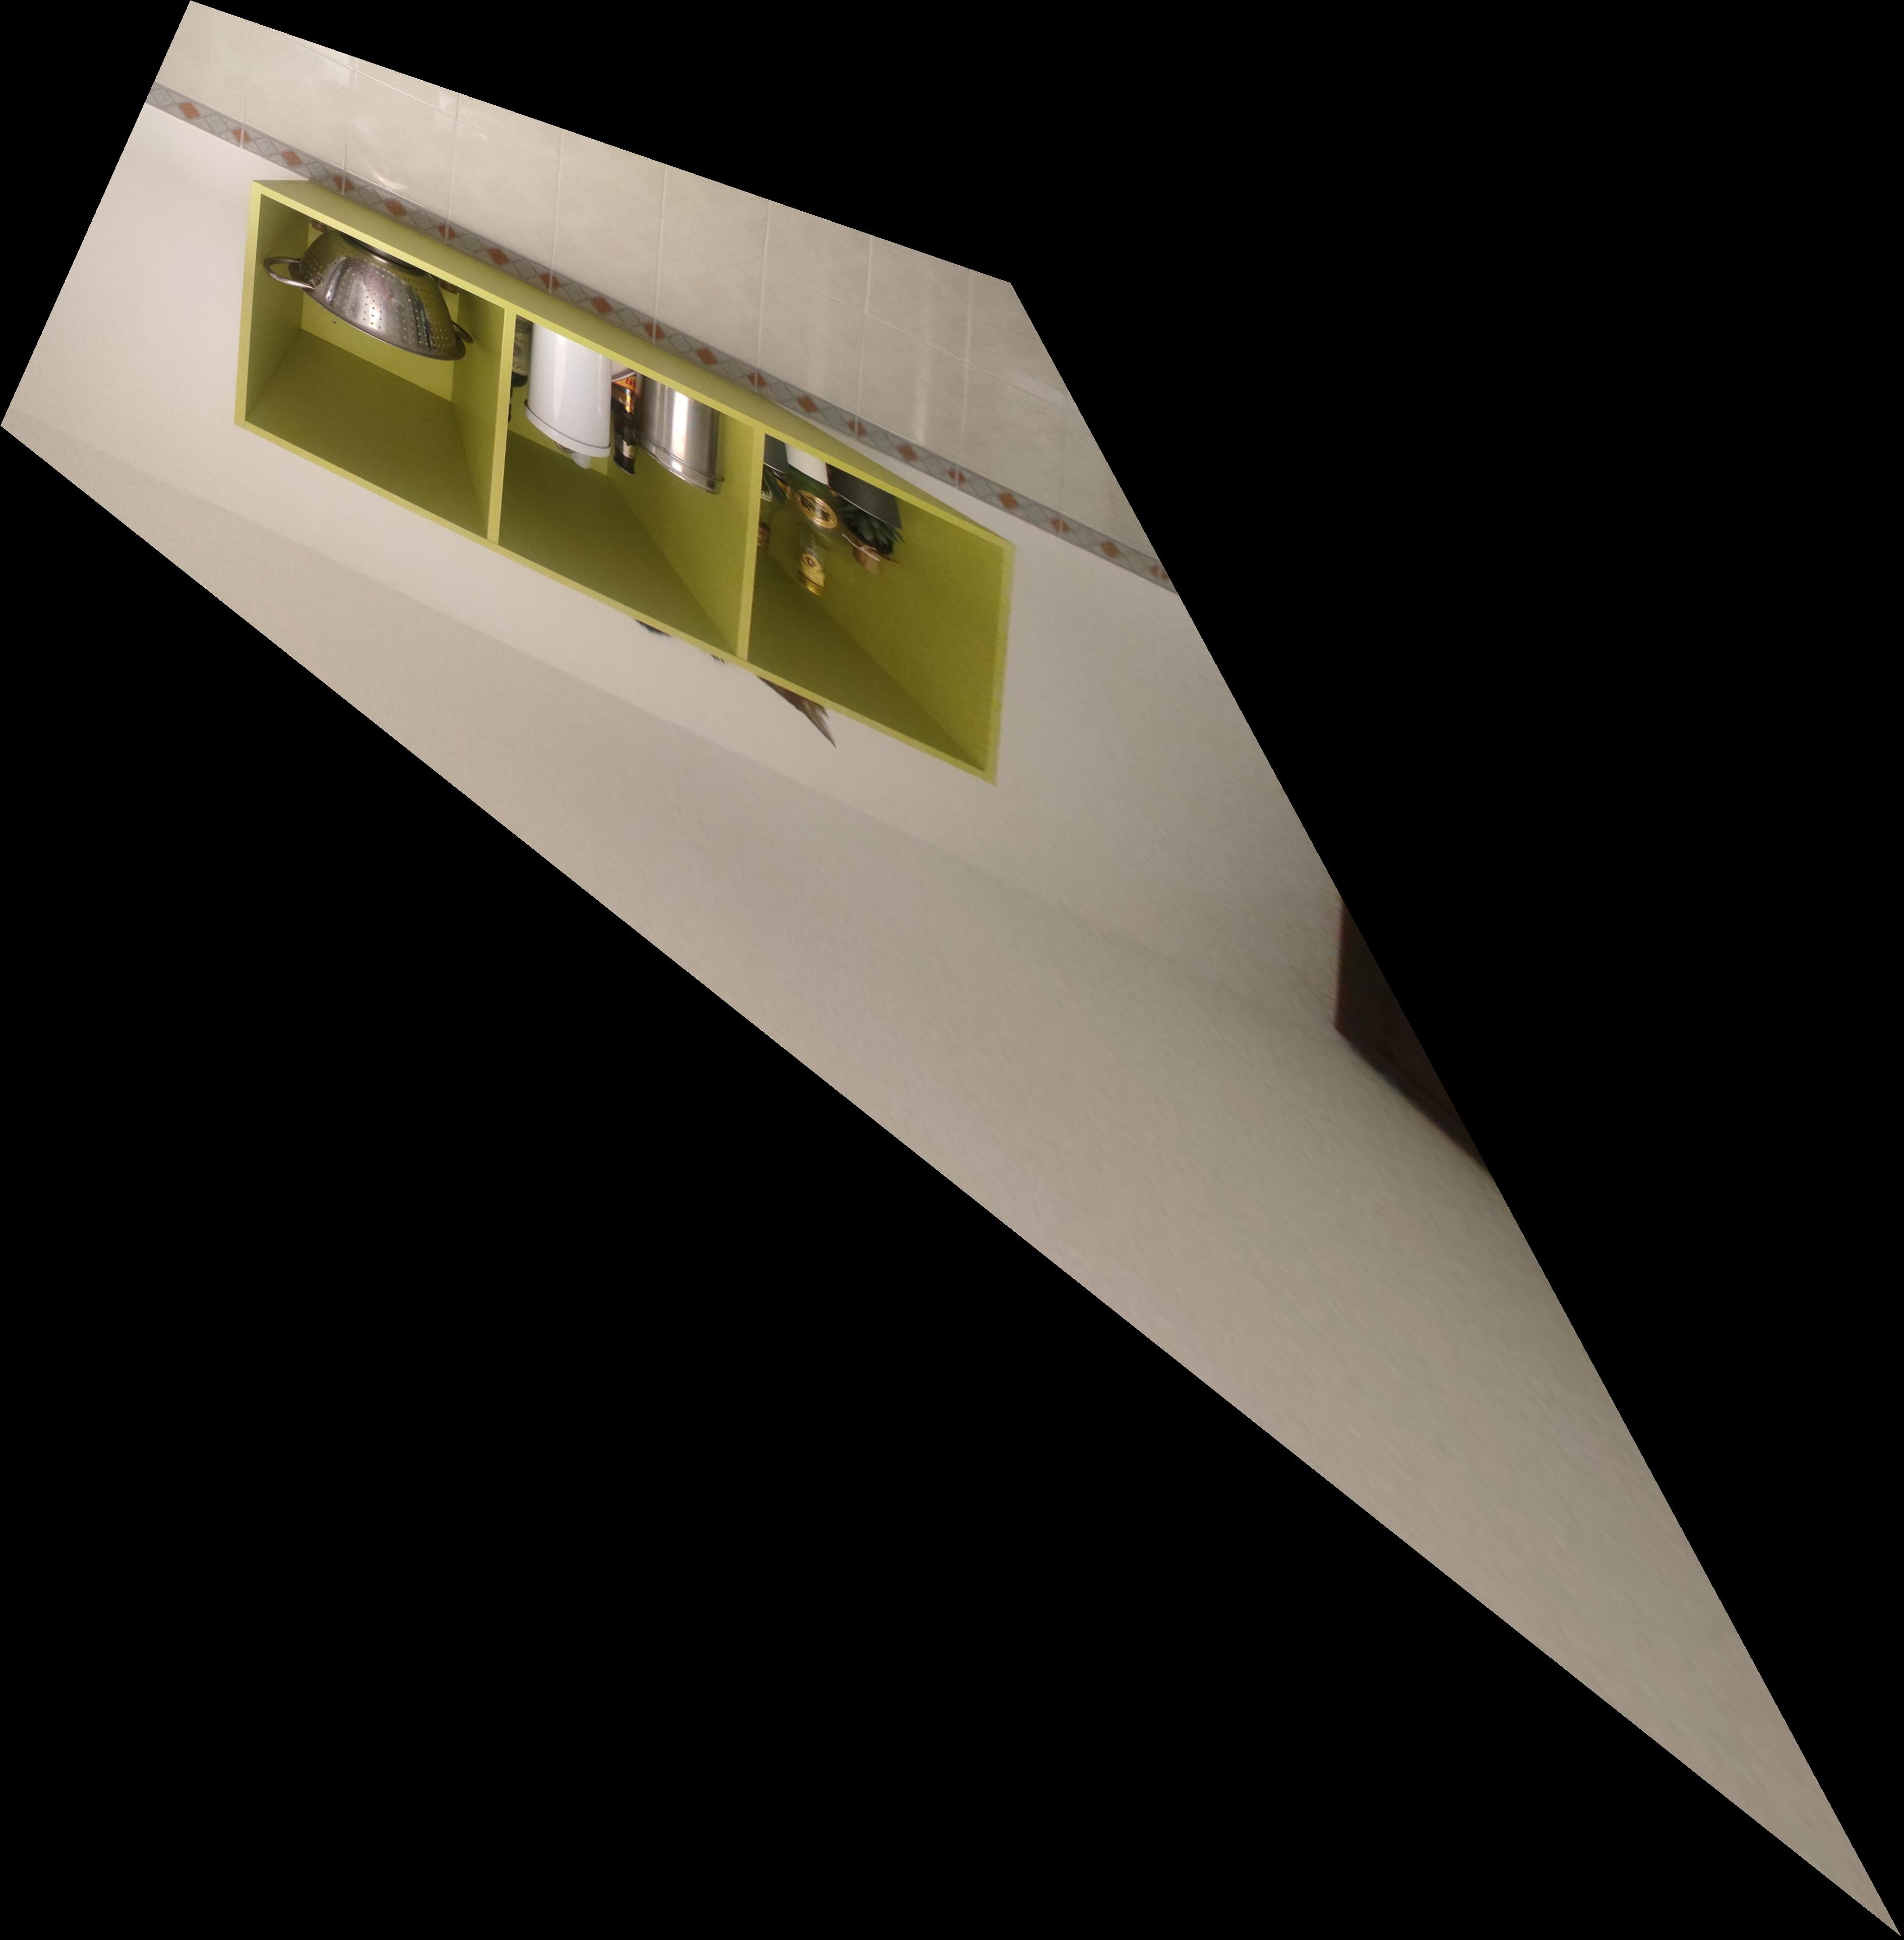
\includegraphics[width=0.95\linewidth]{img/G3/verticalReconstructionK.jpg}
    \caption{Reconstructed vertical plane using $K$}
    \label{fig:verticalRectK}
\end{figure}

\subsection{Estimation of height}
Following the same approach used to determine the depth of the parallelepiped, we can measure $\cos\gamma$ using formula \ref{eq:1} shown in the figure. Knowing that $l_x$ and $h_y$ should form a right angle and given $l = 1 \, \mathrm{m}$, we can compute the numerical value of the height as:

\[
h = l \sqrt{1 - \cos^2\gamma}
\]

Before proceeding with the numerical computation of $h$, it is crucial to verify, in the rectified image, whether the angle between $l$ and $h$ is indeed a right angle. Using a simple program to calculate the angle between two lines, we can verify that $l$ and $h$ are not perfectly perpendicular. This discrepancy arises due to numerical instability and inaccuracies in the matrix $K$.

\subsubsection{2D Reconstruction of the Vertical Plane}
In order to obtain a more precise reconstruction of the vertical plane, we follow the typical approach, using metric-stratified method, selecting $l$ and $m$ lines from the provided image in order to build the affine rectified image and finally selecting, from the obtained result, two pairs of orthogonal and independent lines as shown in the following pictures:

\begin{figure}[H]
     \centering
     \begin{subfigure}[b]{0.45\textwidth}
         \centering
         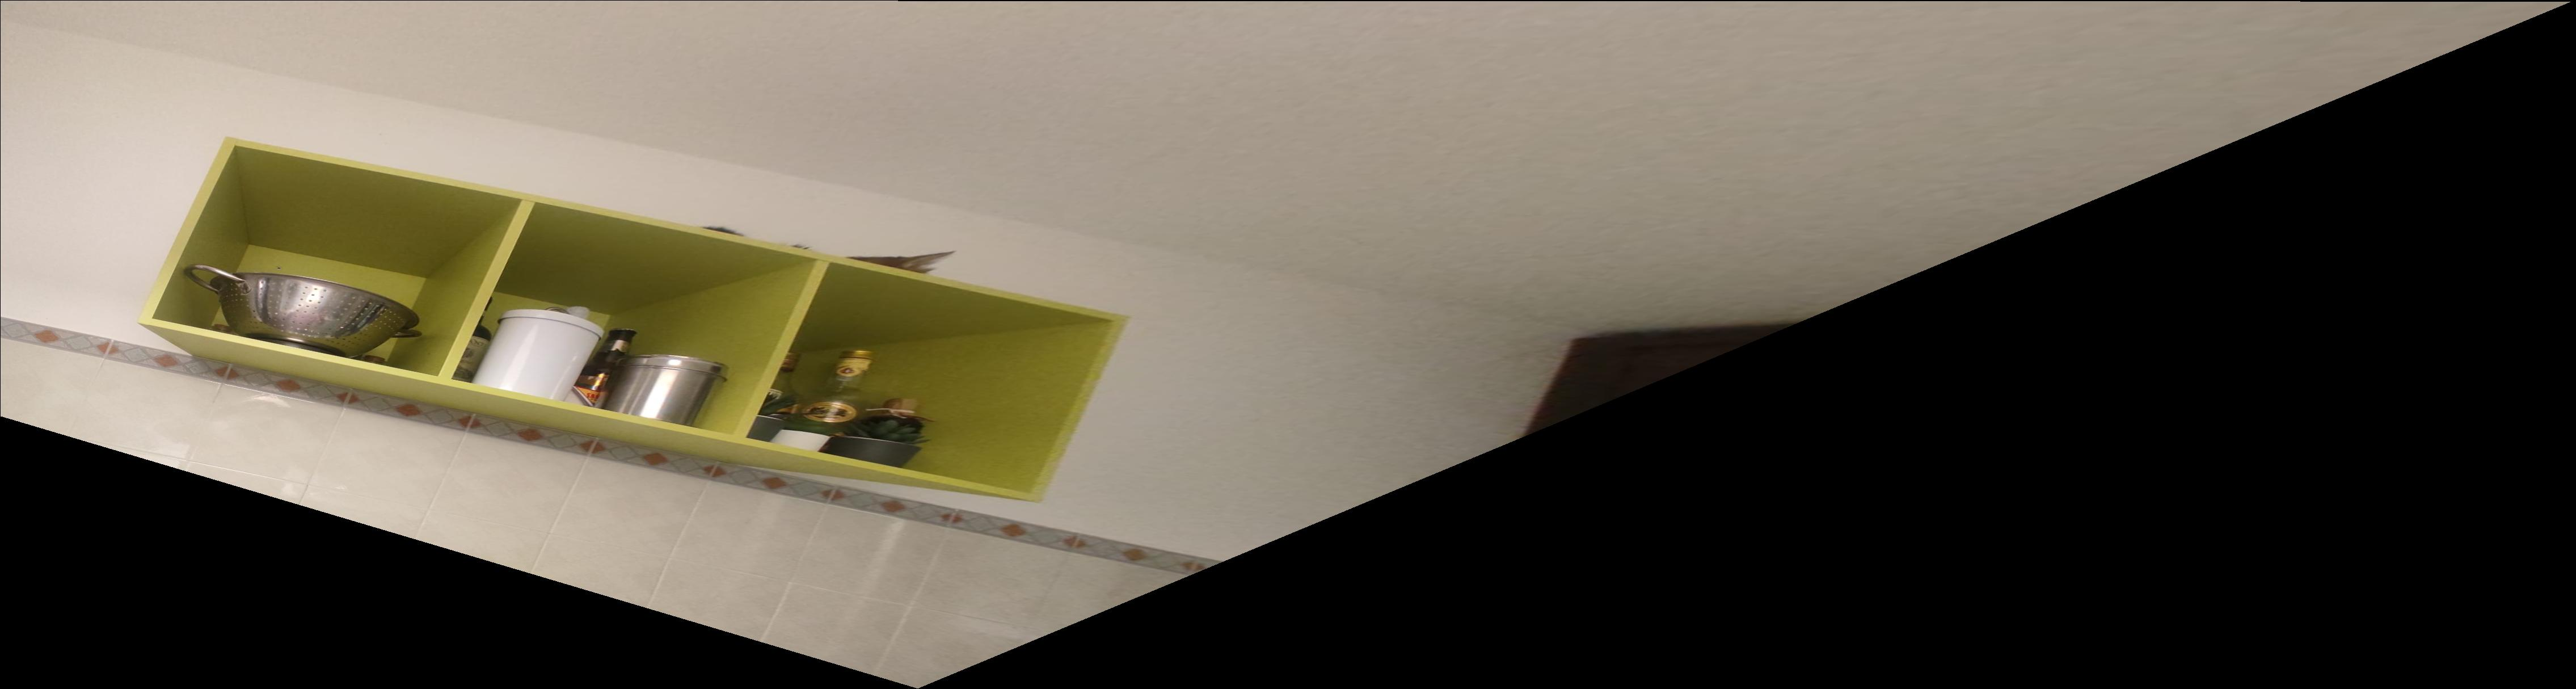
\includegraphics[width=\textwidth]{img/G3/affineVertRectification.jpg}
         \caption{Affine Rectification}
     \end{subfigure}
     \hfill
     \begin{subfigure}[b]{0.45\textwidth}
         \centering
         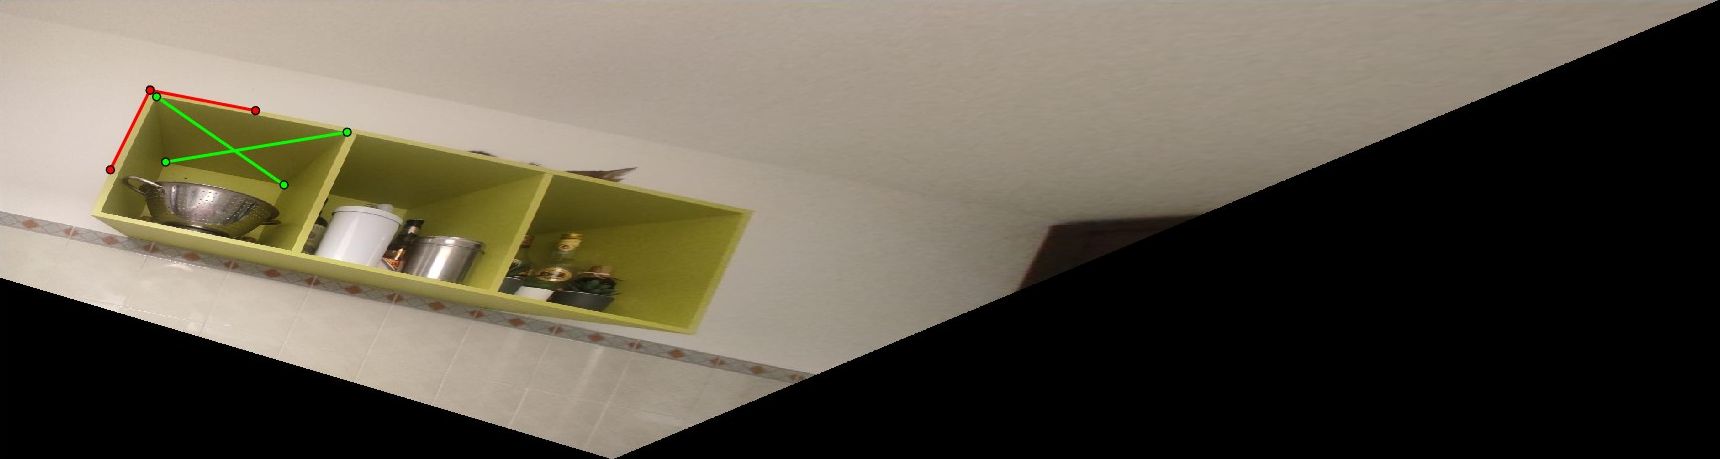
\includegraphics[width=\textwidth]{img/G3/affineWithLines.png}
         \caption{Pairs of orthogonal and independent lines}
         \label{pairOrthogonalLines}
     \end{subfigure}
\end{figure}

Note that the lines in Figure \ref{pairOrthogonalLines} can be selected because, as shown in (\ref{square}), the green lines are the diagonals of a square and are therefore orthogonal.

The rectified image obtained is:
\begin{figure}[H]
    \centering
    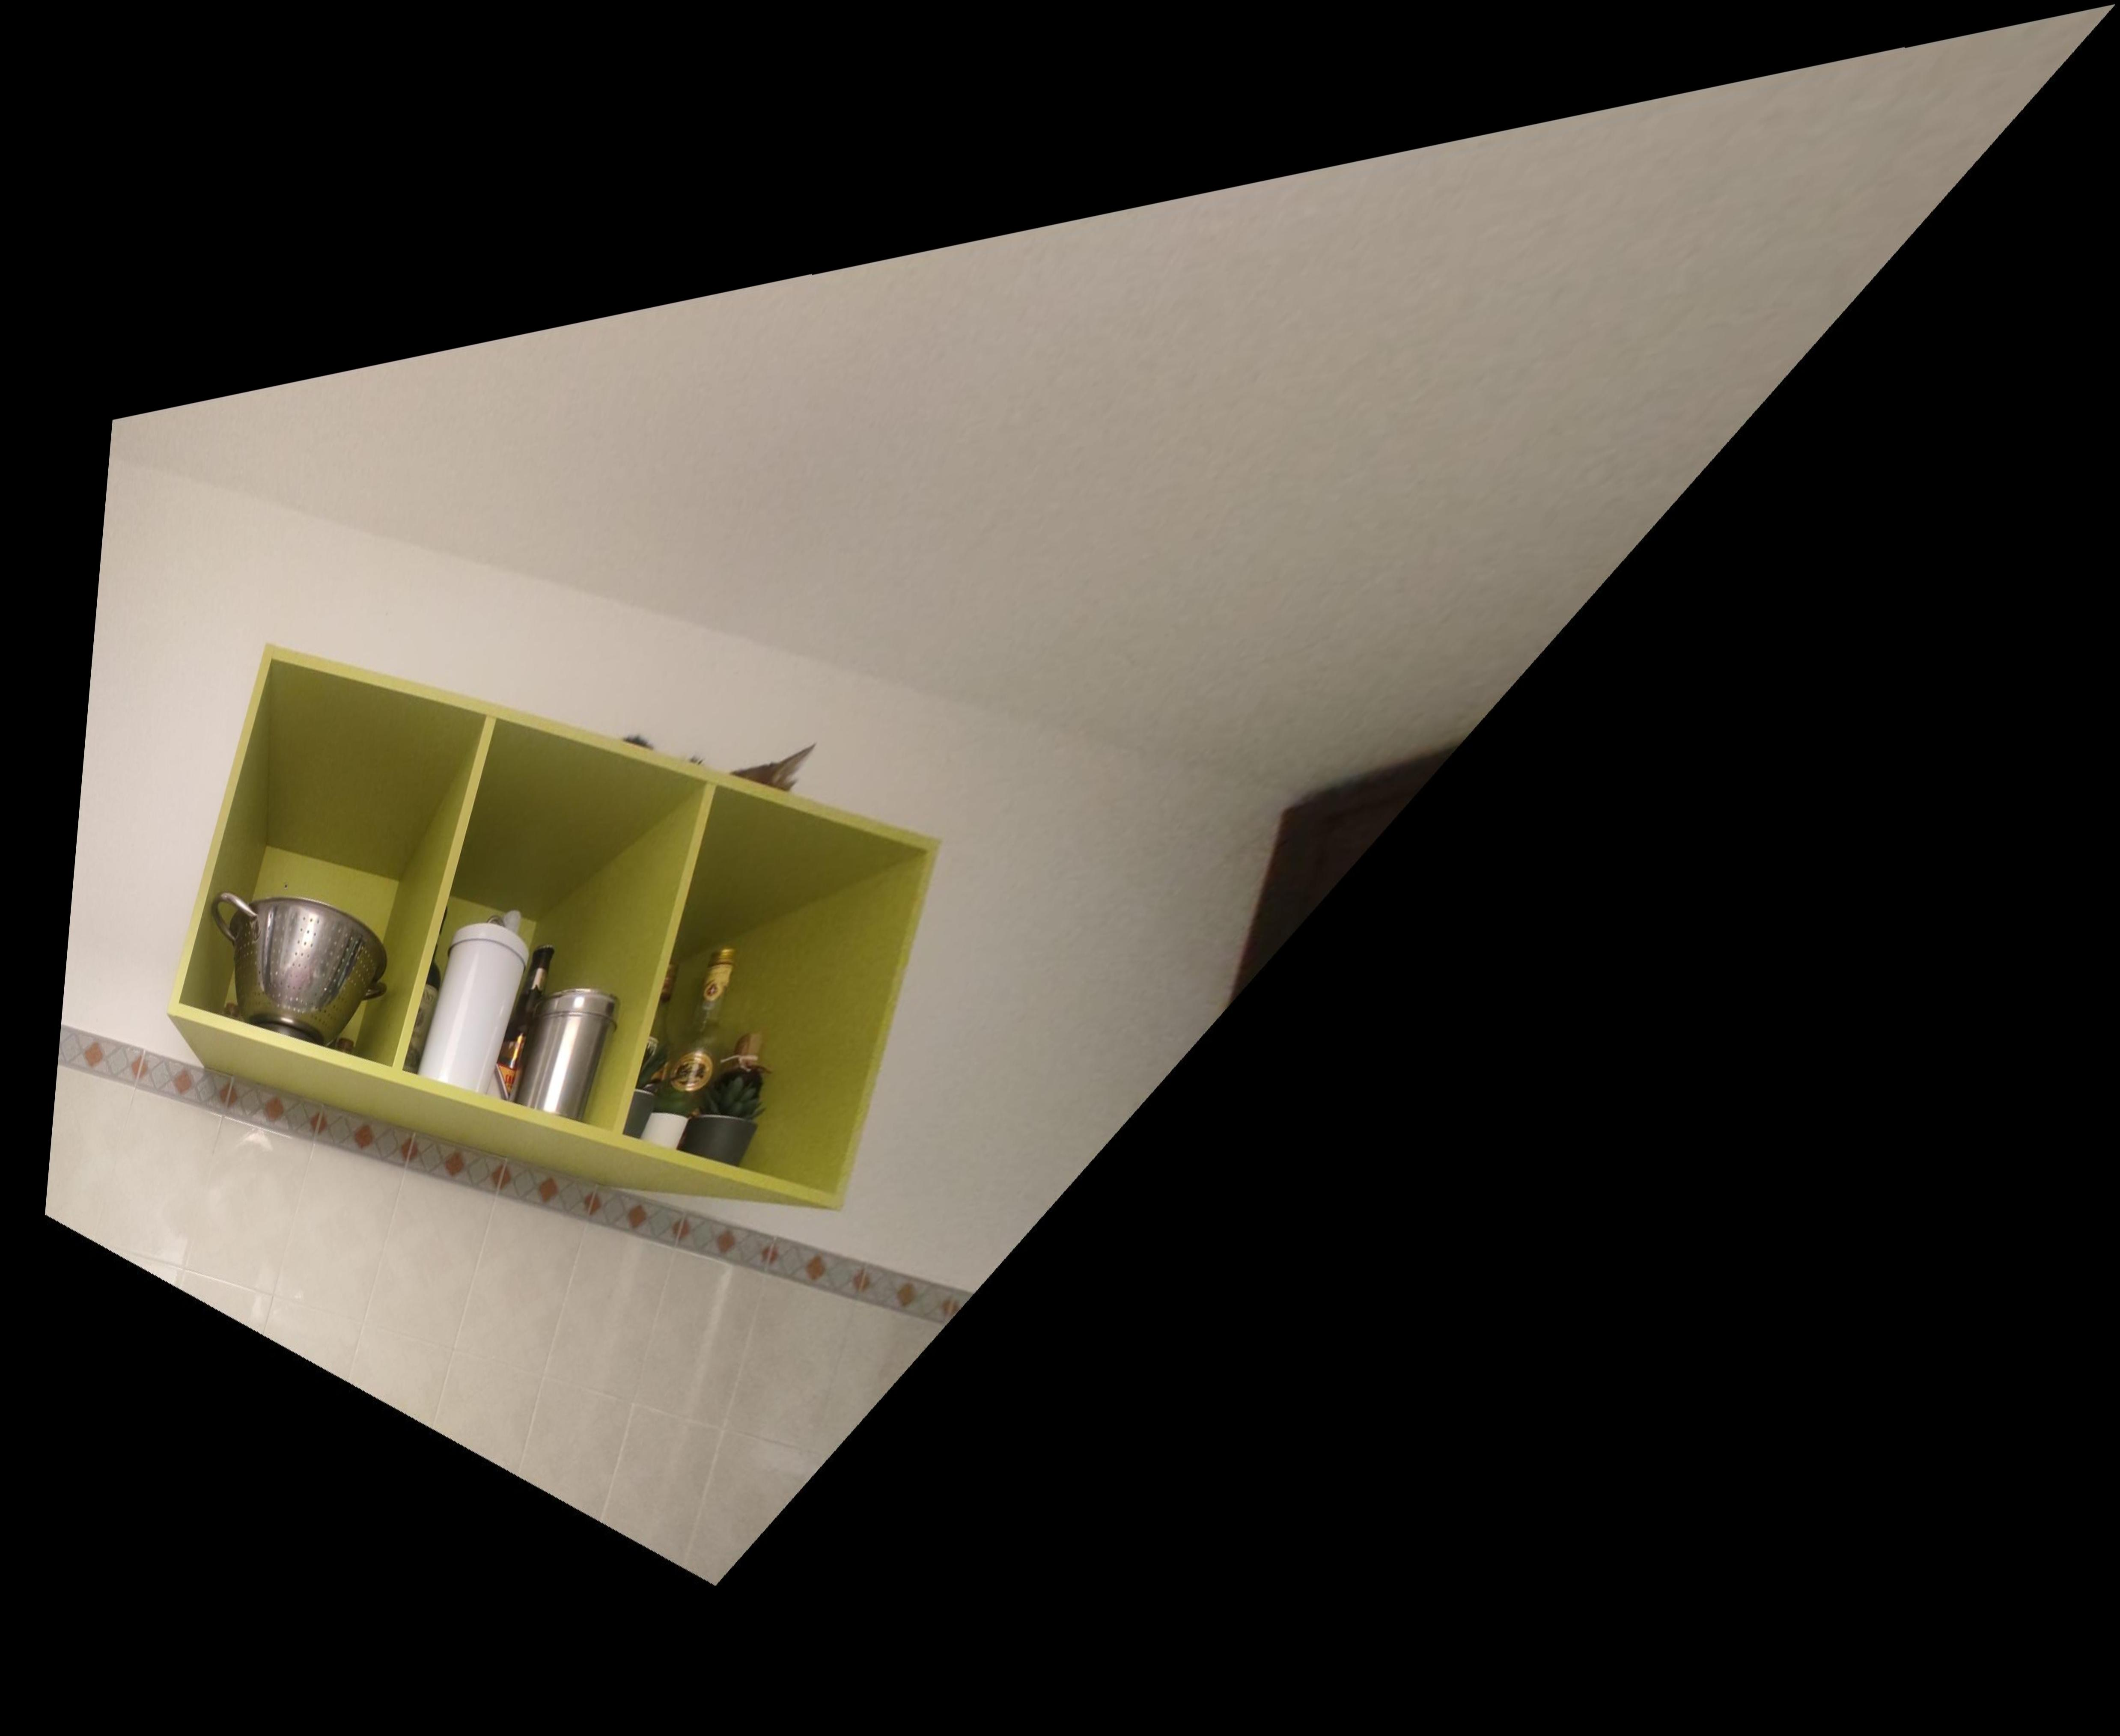
\includegraphics[width=0.75\linewidth]{img/G3/verticalRectificationMetric.jpg}
    \caption{Vertical Rectification}
    \label{fig:verticalRectMetric}
\end{figure}

\subsubsection{Compute $h$}
The obtained result is slightly improved compared to the previous one, as the computed angle between the $l$ and $h$ lines is very close to $90^\circ$. This allows us to calculate a more accurate numerical value for the height of the parallelepiped. The same method used to determine its depth, detailed in Section \ref{estimationDepth}, is applied here. Using the Pythagorean theorem for a right triangle, the $l$ and $h$ lines are defined as the two catheti, we found:

$$h \approx 0.5 \, m$$